\chapter{Grundlagen}
\label{cha:Grundlagen}

\section{MQTT (Message Queue Telemetry Transport)}

\subsection{Allgemein}
Bei MQTT\nomenclature{MQTT}{Message Queue Telemetry Transport} handelt es sich um ein einfaches TCP/IP basiertes Nachrichtenprotokoll, das auf den Bereich Mobile und Internet of Things zugeschnitten ist. MQTT ist gerade im Bereich der Homeautomation sehr beliebt.

Ziele von MQTT sind neben einer hohen Zuverlässigkeit ein sparsamer Umgang mit Bandbreite und Ressourcen. Dadurch eignet sich MQTT auch zur Kommunikation mit mobilen Geräten bei denen Bandbreite und Ressourcen knapp sind.

\subsection{Publish/Subscribe Verfahren}
Der Nachrichtenaustausch bei MQTT funktioniert über das Publish/Subscribe Muster. Bei Publish/Subscribe kommuniziert der Sender der Nachricht nicht direkt mit dem Empfänger, sondern wendet sich an einen Broker, welcher die Zustellung der Nachricht übernimmt. Der Broker entkoppelt so den Sender vom Empfänger der Nachrichten.

\subsection{MQTTS (Message Queue Telemetry Transport Secure)}
Bei MQTTS\nomenclature{MQTT}{Message Queue Telemetry Transport Secure} wird die Kommunikation mit TLS/SSL verschlüsselt. Damit wird ein abhören der Nachrichten erschwert.

\section{TLS (Transport Layer Security)}
TLS\nomenclature{TLS}{Transport Layer Security} (Vorgänger SSL[Secure Sockets Layer])\nomenclature{SSL}{Secure Sockets Layer} ist ein Verschlüsselungsprotokoll zur Verschlüsselung einer Kommunikation. Dabei werden am Anfang Zertifikate zwischen zwei Kommunikationspartnern ausgetauscht mittels eines public key. Dabei identifizieren sich beide nacheinander, bevor dann eine verschlüsselte Verbindung aufgebaut ist.


\section{ESP32}
Der ESP32 wird von Espressif hergestellt und besitzt ein schon eingebautes WLAN/Bluetooth Modul. Damit kann er entweder ein eigenes WLAN\nomenclature{WLAN}{Wireless Local Area Network} Netzwerk aufbauen, oder mit einem vorhandenen Netzwerk kommunizieren, ohne zusätzliche Shields zu benötigen, wie ein Arduino. Der Mikrocontroller kann mit entsprechenden Librarys in der Arduino IDE programmiert werden, oder in der ESP IDF Umgebung\footnote{siehe Kapitel~\ref{cha:Installation_IDF}}.

Abbildung~\ref{fig:esp32} zeigt den Aufbau eines ESP32. Auf der linken Seite sind alle kompatiblen Protokolle für die Pins aufgelistet. Interessant ist dabei auch, dass der ESP32 zwei Cores besitzt mit denen zwei Tasks gleichzeitig ausgeführt werden können. Dadurch wird Multi Threading möglich. Zusätzlich ist der Mikrocontroller mit einer Ultra Low Power Consumption ausgestattet, wodurch ein sehr stromsparender Betrieb möglich wird. Damit ist der ESP32 perfekt für Internet of Things (IoT) Anwendungen geeignet.

\begin{figure}[hbt]
	\centering
	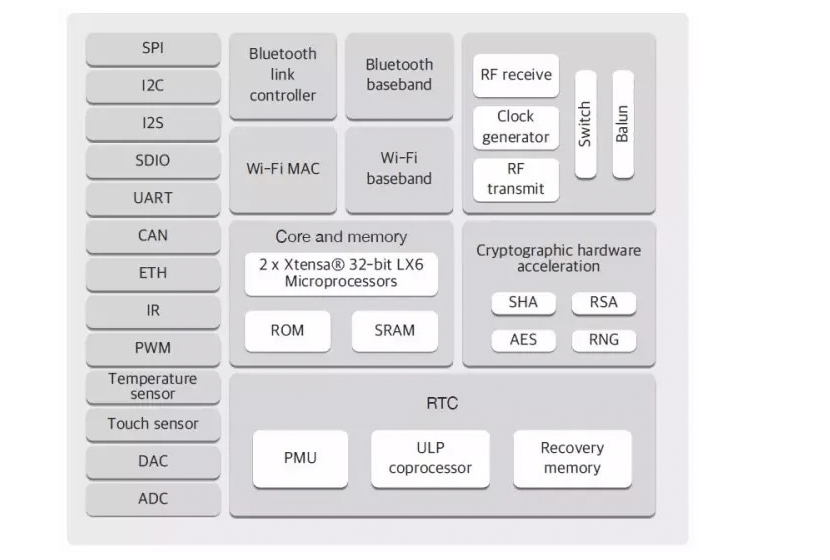
\includegraphics[width=0.7\linewidth]{images/esp32}
	\caption[ESP32 Aufbau]{Aufbau eines ESP32.}
	\label{fig:esp32}
\end{figure}
